\documentclass[11pt,a4paper]{article}
\usepackage[utf8]{inputenc}
\usepackage[T1]{fontenc}
\IfFileExists{romanian.ldf}{\usepackage[romanian]{babel}}{}
\usepackage{lmodern}
\usepackage[margin=2.2cm]{geometry}
\usepackage{xcolor}
\usepackage{listings}
\usepackage{booktabs}
\usepackage{enumitem}
\usepackage{fancyhdr}
\usepackage[most]{tcolorbox}
\usepackage[hidelinks]{hyperref}

\definecolor{codebg}{RGB}{247,247,250}
\definecolor{kw}{RGB}{0,70,150}
\definecolor{cm}{RGB}{90,120,90}
\definecolor{st}{RGB}{160,60,30}

\lstset{
  basicstyle=\ttfamily\small,
  backgroundcolor=\color{codebg},
  keywordstyle=\color{kw}\bfseries,
  commentstyle=\color{cm}\itshape,
  stringstyle=\color{st},
  numbers=left, numberstyle=\tiny\color{gray},
  frame=single, rulecolor=\color{gray!40},
  breaklines=true, columns=fullflexible, keepspaces=true,
  showstringspaces=false, tabsize=4,
  literate={ă}{{\u{a}}}1 {â}{{\^{a}}}1 {î}{{\^{\i}}}1 {ș}{{\c{s}}}1 {ț}{{\c{t}}}1
}

\newtcolorbox{terminal}[1][]{colback=black!85,colframe=black!60,coltext=white,
  fontupper=\ttfamily\small,boxrule=0.4pt,arc=2pt,left=4pt,right=4pt,top=3pt,bottom=3pt,title={#1},
  fonttitle=\sffamily\small\bfseries,colbacktitle=black!60}
\newtcolorbox{answer}{colback=blue!3,colframe=blue!40!black,boxrule=0.4pt,arc=2pt,
  left=6pt,right=6pt}

\pagestyle{fancy}
\fancyhf{}
\lhead{Sisteme de Operare -- FCIM, UTM}
\rhead{Ciur Alexandrina}
\cfoot{\thepage}
\usepackage{tikz}
\usetikzlibrary{arrows.meta,positioning}

\begin{document}

\begin{titlepage}
\centering
{\large Ministerul Educației și Cercetării al Republicii Moldova\\
Universitatea Tehnică a Moldovei\\
Facultatea Calculatoare, Informatică și Microelectronică\par}
\vspace{5cm}
{\LARGE\bfseries RAPORT\par}
\vspace{0.6cm}
{\Large Lucrarea de laborator nr.~12\par}
\vspace{0.4cm}
{\large la disciplina \textit{Sisteme de Operare}\par}
\vspace{0.6cm}
{\Large\bfseries Producer, Consumer and the Other Tools (Linux)\par}
\vfill
\begin{flushright}
\begin{tabular}{ll}
A efectuat: & Ciur Alexandrina \\
A verificat: & \rule{4.5cm}{0.4pt} \\
\end{tabular}
\end{flushright}
\vspace{2cm}
{\large Chișinău, 2026\par}
\end{titlepage}

\section*{Scopul lucrării}
În laboratorul 11 semafoarele au fost folosite pe rând: ca lock, ca semnal și ca numărător. Acum instrumentele lucrează
împreună. Rezolvăm cele două probleme clasice de sincronizare, \textbf{producător--consumator} și
\textbf{cititori--scriitori}, folosim \textbf{variabila de condiție} și construim, apoi eliminăm, un
\textbf{deadlock}.

\section*{Noțiuni teoretice}
\begin{itemize}[leftmargin=*]
  \item \textbf{Buffer limitat (producător--consumator)}: două semafoare numără sloturile libere (\texttt{empty}) și
        ocupate (\texttt{full}), iar un mutex protejează bufferul. Așa funcționează și \texttt{pipe}-urile din kernelul Unix.
  \item \textbf{Variabila de condiție} (\texttt{pthread\_cond\_t}): locul în care un thread doarme până când alt thread
        anunță o schimbare. \texttt{pthread\_cond\_wait} eliberează mutexul, adoarme și reia mutexul înainte să revină.
        Starea propriu-zisă e păstrată într-o variabilă obișnuită.
  \item \textbf{Cititori--scriitori}: mai mulți cititori pot citi simultan, dar un scriitor trebuie să fie singur.
  \item \textbf{Deadlock}: un set de thread-uri în care fiecare așteaptă o resursă ținută de altul. Condițiile Coffman
        sunt excluderea mutuală, hold-and-wait, fără preempțiune și \emph{așteptarea circulară}.
  \item \textbf{Starvation}: un thread nu e blocat definitiv, dar nu primește niciodată resursa.
\end{itemize}

%======================================================================
\section{Partea 1 -- Producător și consumator}
\begin{lstlisting}[language=C,title={\texttt{prodcons.c}}]
/* prodcons.c - producer and consumer around a buffer of 4 slots.
 *   empty = free slots (starts at SIZE), full = filled slots (starts at 0), lock = the buffer itself.
 * Build: gcc -Wall -pthread -o prodcons prodcons.c
 */
#include <stdio.h>
#include <unistd.h>
#include <pthread.h>
#include <semaphore.h>

#define SIZE 4
#define ITEMS 8

int buf[SIZE];
int in = 0, out = 0, count = 0;         /* count only for printing */
sem_t empty, full;
pthread_mutex_t lock = PTHREAD_MUTEX_INITIALIZER;

void *producer(void *arg) {
    for (int item = 1; item <= ITEMS; item++) {
        sem_wait(&empty);               /* wait for a free slot */
        pthread_mutex_lock(&lock);
        buf[in] = item;
        in = (in + 1) % SIZE;
        count++;
        printf("put %d    (in buffer: %d)\n", item, count);
        pthread_mutex_unlock(&lock);
        sem_post(&full);                /* one more filled slot */
    }
    return NULL;
}

void *consumer(void *arg) {
    for (int k = 0; k < ITEMS; k++) {
        sem_wait(&full);                /* wait for something to take */
        pthread_mutex_lock(&lock);
        int item = buf[out];
        out = (out + 1) % SIZE;
        count--;
        printf("            take %d   (in buffer: %d)\n", item, count);
        pthread_mutex_unlock(&lock);
        sem_post(&empty);               /* one more free slot */
        usleep(300000);                 /* the consumer is slow */
    }
    return NULL;
}

int main(void) {
    sem_init(&empty, 0, SIZE);
    sem_init(&full, 0, 0);
    pthread_t p, c;
    pthread_create(&c, NULL, consumer, NULL);
    pthread_create(&p, NULL, producer, NULL);
    pthread_join(p, NULL);
    pthread_join(c, NULL);
    sem_destroy(&empty);
    sem_destroy(&full);
    return 0;
}
\end{lstlisting}

\begin{terminal}[Rulare]
\begin{verbatim}
$ ./prodcons
put 1    (in buffer: 1)
put 2    (in buffer: 2)
put 3    (in buffer: 3)
put 4    (in buffer: 4)
            take 1   (in buffer: 3)
put 5    (in buffer: 4)
            take 2   (in buffer: 3)
put 6    (in buffer: 4)
            take 3   (in buffer: 3)
put 7    (in buffer: 4)
            take 4   (in buffer: 3)
put 8    (in buffer: 4)
            take 5   (in buffer: 3)
            take 6   (in buffer: 2)
            take 7   (in buffer: 1)
            take 8   (in buffer: 0)
\end{verbatim}
\end{terminal}

\begin{terminal}[Mutexul luat ÎNAINTE de sem\_wait(\&empty)]
\begin{verbatim}
$ timeout 5 ./prodcons; echo "exit code: $?"   # versiunea modificata
put 1    (in buffer: 1)
put 2    (in buffer: 2)
put 3    (in buffer: 3)
put 4    (in buffer: 4)
exit code: 124
\end{verbatim}
\end{terminal}

\subsection*{Observații}
\begin{answer}
\textbf{1. Ce îl oprește pe producător la 4.} Apelul \texttt{sem\_wait(\&empty)}. \texttt{empty} pornește de la
\texttt{SIZE = 4}. După 4 elemente ajunge la 0, iar producătorul doarme până când consumatorul eliberează un slot cu
\texttt{sem\_post(\&empty)}.

\medskip
\textbf{2. Cine așteaptă la început.} \textbf{Consumatorul}, în \texttt{sem\_wait(\&full)}: \texttt{full} începe de la 0
(bufferul e gol), deci consumatorul doarme până la primul \texttt{sem\_post(\&full)} al producătorului.

\medskip
\textbf{3. Lock înainte de \texttt{sem\_wait(\&empty)}.} Apare \textbf{deadlock} când bufferul e plin. Producătorul ia
mutexul, apoi adoarme în \texttt{sem\_wait(\&empty)} \emph{ținând mutexul}. Consumatorul trece de
\texttt{sem\_wait(\&full)}, dar se blochează la \texttt{pthread\_mutex\_lock}. Fiecare așteaptă ceva ce doar celălalt
poate elibera. Regula: nu adormi pe un semafor ținând un lock. Ordinea corectă e întâi semaforul, apoi mutexul.
\end{answer}

%======================================================================
\section{Partea 2 -- Variabila de condiție}
Problema din \texttt{order.c} (Lab 11) rezolvată altfel: cu un mutex, o variabilă \texttt{ready} și o variabilă de
condiție.

\begin{lstlisting}[language=C,title={\texttt{condvar.c}}]
/* condvar.c - the order.c problem, solved with a mutex and a condition variable.
 * Build: gcc -Wall -pthread -o condvar condvar.c
 */
#include <stdio.h>
#include <string.h>
#include <unistd.h>
#include <pthread.h>

char message[32];
int ready = 0;                                  /* the condition itself */
pthread_mutex_t lock = PTHREAD_MUTEX_INITIALIZER;
pthread_cond_t changed = PTHREAD_COND_INITIALIZER;

void *writer(void *arg) {
    sleep(1);
    pthread_mutex_lock(&lock);
    strcpy(message, "hello");
    ready = 1;
    printf("A: message written\n");
    pthread_cond_signal(&changed);              /* wake one waiter */
    pthread_mutex_unlock(&lock);
    return NULL;
}

void *reader(void *arg) {
    pthread_mutex_lock(&lock);
    while (!ready) {                            /* while, not if: re-check after waking */
        printf("B: not ready, I sleep\n");
        pthread_cond_wait(&changed, &lock);     /* unlocks, sleeps, locks again */
    }
    printf("B: I read \"%s\"\n", message);
    pthread_mutex_unlock(&lock);
    return NULL;
}

int main(void) {
    pthread_t a, b;
    pthread_create(&b, NULL, reader, NULL);
    pthread_create(&a, NULL, writer, NULL);
    pthread_join(a, NULL);
    pthread_join(b, NULL);
    return 0;
}
\end{lstlisting}

\begin{terminal}[Rulare (cu while și cu if: același rezultat)]
\begin{verbatim}
$ ./condvar
B: not ready, I sleep
A: message written
B: I read "hello"
\end{verbatim}
\end{terminal}

\subsection*{Observații}
\begin{answer}
\textbf{1. Cine reține că mesajul e gata.} Variabila \textbf{\texttt{ready}}, protejată de mutexul \texttt{lock}.
Variabila de condiție nu are memorie: un \texttt{signal} trimis când nu așteaptă nimeni se pierde. La semafor, starea era
chiar valoarea lui.

\medskip
\textbf{2. Cu \texttt{if (!ready)}.} Funcționează și aici, cu același output, pentru că există un singur scriitor și un
singur cititor.

\medskip
\textbf{3. De ce \texttt{while}.} (a)~\emph{Spurious wakeup}: POSIX permite ca \texttt{pthread\_cond\_wait} să se
întoarcă fără niciun \texttt{signal}, cu \texttt{ready} încă 0. (b)~Cu mai mulți cititori, alt thread poate prinde
mutexul primul și poate consuma condiția (pune \texttt{ready} înapoi la 0) înainte ca thread-ul nostru să revină. Cu
\texttt{while}, condiția e reverificată după fiecare trezire.
\end{answer}

%======================================================================
\section{Partea 3 -- Cititori și scriitori}
\begin{lstlisting}[language=C,title={\texttt{readers.c}}]
/* readers.c - readers and writers with two semaphores.
 *   Many readers may read together; a writer must be alone.
 * Build: gcc -Wall -pthread -o readers readers.c
 */
#include <stdio.h>
#include <unistd.h>
#include <pthread.h>
#include <semaphore.h>

#define READERS 3
#define WRITERS 2

int value = 0;                  /* the shared data */
int readers = 0;                /* how many are reading now */
sem_t rlock;                    /* protects the counter readers */
sem_t room;                     /* 1 = the room is free for a writer */

void *reader(void *arg) {
    long id = (long)arg;
    sem_wait(&rlock);
    if (++readers == 1)         /* the first reader in locks out the writers */
        sem_wait(&room);
    sem_post(&rlock);

    printf("reader %ld reads %d   (readers inside: %d)\n", id, value, readers);
    usleep(200000);

    sem_wait(&rlock);
    if (--readers == 0)         /* the last reader out lets the writers in */
        sem_post(&room);
    sem_post(&rlock);
    return NULL;
}

void *writer(void *arg) {
    long id = (long)arg;
    sem_wait(&room);            /* alone in the room */
    value += 10;
    printf("writer %ld writes %d   (alone)\n", id, value);
    usleep(200000);
    sem_post(&room);
    return NULL;
}

int main(void) {
    sem_init(&rlock, 0, 1);
    sem_init(&room, 0, 1);
    pthread_t r[READERS], w[WRITERS];
    pthread_create(&w[0], NULL, writer, (void *)1L);
    for (long i = 0; i < READERS; i++)
        pthread_create(&r[i], NULL, reader, (void *)(i + 1));
    pthread_create(&w[1], NULL, writer, (void *)2L);
    for (int i = 0; i < READERS; i++) pthread_join(r[i], NULL);
    for (int i = 0; i < WRITERS; i++) pthread_join(w[i], NULL);
    return 0;
}
\end{lstlisting}

\begin{terminal}[Rulare]
\begin{verbatim}
$ ./readers
writer 1 writes 10   (alone)
reader 1 reads 10   (readers inside: 1)
reader 2 reads 10   (readers inside: 2)
reader 3 reads 10   (readers inside: 3)
writer 2 writes 20   (alone)
\end{verbatim}
\end{terminal}

\subsection*{Observații}
\begin{answer}
\textbf{1. Cele două linii.} \texttt{if (++readers == 1) sem\_wait(\&room);}: doar \emph{primul} cititor încuie camera,
iar ceilalți intră liber. \texttt{if (--readers == 0) sem\_post(\&room);}: doar \emph{ultimul} cititor o descuie.
Scriitorul ia \texttt{room} direct, deci e mereu singur.

\medskip
\textbf{2. De ce \texttt{rlock}.} \texttt{++readers}/\texttt{--readers} sunt load/add/store, deci au aceeași problemă ca
\texttt{counter++}. Fără \texttt{rlock}, doi cititori pot crede amândoi că sunt „primii” (al doilea se blochează inutil în
\texttt{sem\_wait(\&room)}) sau „ultimii” (dublu \texttt{sem\_post}, deci \texttt{room = 2} și un scriitor intră peste
cititori). Se poate întâmpla și ca niciunul să nu vadă 0, iar atunci camera nu se mai eliberează și scriitorii așteaptă
la infinit.

\medskip
\textbf{3. Cititori care sosesc continuu.} Writer 2 suferă de \textbf{starvation}: cât timp mai e un cititor înăuntru,
\texttt{readers} nu ajunge la 0, \texttt{room} nu se eliberează, iar scriitorul așteaptă la nesfârșit, deși sistemul nu e
în deadlock. Soluția favorizează cititorii.
\end{answer}

%======================================================================
\section{Partea 4 -- Construim un deadlock, apoi îl eliminăm}
\subsection{Versiunea care se blochează}
\begin{lstlisting}[language=C,title={\texttt{deadlock\_original.c}}]
/* deadlock_original.c - two threads, two mutexes, taken in opposite order (the BROKEN version).
 * Build: gcc -Wall -pthread -o deadlock_original deadlock_original.c
 * Run:   timeout 5 ./deadlock_original; echo "exit code: $?"      (124 = killed by timeout)
 */
#include <stdio.h>
#include <unistd.h>
#include <pthread.h>

pthread_mutex_t A = PTHREAD_MUTEX_INITIALIZER;
pthread_mutex_t B = PTHREAD_MUTEX_INITIALIZER;

void *one(void *arg) {
    pthread_mutex_lock(&A);
    printf("one: I have A, I want B\n");
    sleep(1);
    pthread_mutex_lock(&B);             /* waits for two */
    printf("one: I have both\n");
    pthread_mutex_unlock(&B);
    pthread_mutex_unlock(&A);
    return NULL;
}

void *two(void *arg) {
    pthread_mutex_lock(&B);             /* the fix: lock A first here too */
    printf("two: I have B, I want A\n");
    sleep(1);
    pthread_mutex_lock(&A);             /* waits for one */
    printf("two: I have both\n");
    pthread_mutex_unlock(&A);
    pthread_mutex_unlock(&B);
    return NULL;
}

int main(void) {
    pthread_t t1, t2;
    pthread_create(&t1, NULL, one, NULL);
    pthread_create(&t2, NULL, two, NULL);
    pthread_join(t1, NULL);
    pthread_join(t2, NULL);
    printf("done\n");
    return 0;
}
\end{lstlisting}

\begin{terminal}[Rulare]
\begin{verbatim}
$ timeout 5 ./deadlock_original; echo "exit code: $?"
two: I have B, I want A
one: I have A, I want B
exit code: 124
\end{verbatim}
\end{terminal}

\subsection{Versiunea reparată}
În \texttt{two()} se ia întâi A, apoi B, adică în aceeași ordine ca în \texttt{one()}.
\begin{lstlisting}[language=C,title={\texttt{deadlock.c}}]
/* deadlock.c - two threads, two mutexes - FIXED version.
 * Both threads now take the locks in the SAME order (A, then B), so no circular wait is possible.
 * Build: gcc -Wall -pthread -o deadlock deadlock.c
 * Run:   timeout 5 ./deadlock; echo "exit code: $?"      (0 = finished normally)
 */
#include <stdio.h>
#include <unistd.h>
#include <pthread.h>

pthread_mutex_t A = PTHREAD_MUTEX_INITIALIZER;
pthread_mutex_t B = PTHREAD_MUTEX_INITIALIZER;

void *one(void *arg) {
    pthread_mutex_lock(&A);
    printf("one: I have A, I want B\n");
    sleep(1);
    pthread_mutex_lock(&B);
    printf("one: I have both\n");
    pthread_mutex_unlock(&B);
    pthread_mutex_unlock(&A);
    return NULL;
}

void *two(void *arg) {
    pthread_mutex_lock(&A);             /* the fix: lock A first, the same order as one() */
    printf("two: I have B, I want A\n");
    sleep(1);
    pthread_mutex_lock(&B);             /* then B */
    printf("two: I have both\n");
    pthread_mutex_unlock(&B);
    pthread_mutex_unlock(&A);
    return NULL;
}

int main(void) {
    pthread_t t1, t2;
    pthread_create(&t1, NULL, one, NULL);
    pthread_create(&t2, NULL, two, NULL);
    pthread_join(t1, NULL);
    pthread_join(t2, NULL);
    printf("done\n");
    return 0;
}
\end{lstlisting}

\begin{terminal}[Rulare]
\begin{verbatim}
$ timeout 5 ./deadlock; echo "exit code: $?"
two: I have B, I want A
two: I have both
one: I have A, I want B
one: I have both
done
exit code: 0
\end{verbatim}
\end{terminal}

\subsection*{Observații}
\begin{answer}
\textbf{1. Cercul.} \texttt{one} ține \textbf{A} și așteaptă \textbf{B}; \texttt{two} ține \textbf{B} și așteaptă
\textbf{A}:

\begin{center}
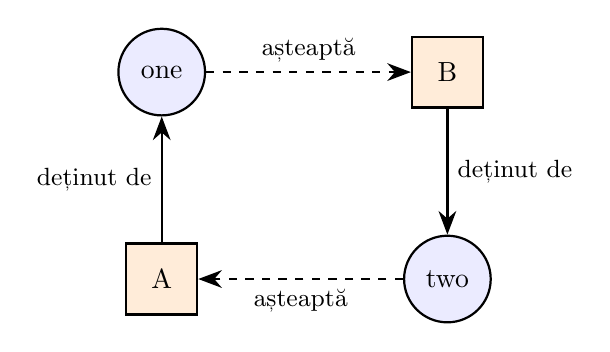
\begin{tikzpicture}[node distance=2.6cm, >={Stealth[length=3mm]},
  thr/.style={circle,draw,thick,minimum size=1.1cm,fill=blue!8},
  res/.style={rectangle,draw,thick,minimum size=0.9cm,fill=orange!15}]
  \node[thr] (one) {one};
  \node[res, right=of one] (B) {B};
  \node[thr, below=1.6cm of B] (two) {two};
  \node[res, below=1.6cm of one] (A) {A};
  \draw[->,thick,dashed] (one) -- node[above]{\small așteaptă} (B);
  \draw[->,thick] (B) -- node[right]{\small deținut de} (two);
  \draw[->,thick,dashed] (two) -- node[below]{\small așteaptă} (A);
  \draw[->,thick] (A) -- node[left]{\small deținut de} (one);
\end{tikzpicture}
\end{center}
Ciclul \texttt{one} $\to$ B $\to$ \texttt{two} $\to$ A $\to$ \texttt{one} este o \emph{așteptare circulară}.

\medskip
\textbf{2. Fără \texttt{sleep(1)}, 10 rulări.} Codurile de ieșire au fost
\texttt{124 0 124 0 0 0 124 0 124 124}, deci programul s-a blocat de 5 ori din 10. \textbf{Nu} se mai blochează mereu:
adesea un thread apucă să ia ambele mutexuri înainte ca celălalt să pornească. Asta e \emph{mai rău}, pentru că bug-ul
devine intermitent: trece testele, apoi blochează programul în producție, sub altă încărcare. E greu de reprodus și de
depanat, pe când cu \texttt{sleep(1)} deadlock-ul era garantat și evident.

\medskip
\textbf{3. De ce aceeași ordine nu dă deadlock.} Dacă toți iau lock-urile în aceeași ordine globală (A înaintea lui B),
cine ține B a trecut deja de A. Nimeni nu poate ține B și aștepta A, deci așteptarea circulară nu se poate forma.
\end{answer}

%======================================================================
\section*{Concluzii}
Am combinat semafoarele cu mutexurile pentru a rezolva problemele clasice de sincronizare. La
\textbf{producător--consumator}, \texttt{empty} și \texttt{full} numără sloturile, iar mutexul protejează bufferul;
ordinea apelurilor contează, pentru că un lock ținut în timp ce dormi pe un semafor produce deadlock. \textbf{Variabila de
condiție} separă starea (\texttt{ready}) de mecanismul de așteptare, iar așteptarea se face mereu într-un \texttt{while}.
Soluția \textbf{cititori--scriitori} permite citiri paralele, dar poate înfometa scriitorii. Am construit un
\textbf{deadlock} cu două mutexuri luate în ordine inversă și l-am eliminat impunând o ordine globală de achiziție. Am
observat și că deadlock-urile nedeterministe sunt cele mai periculoase.

\end{document}
